\subsection{Images}
\label{sec:images}

We continue analyzing images and present the following useful metric
distributions: image size and compressibility, layer reference count, file and
directory counts.

\paragraph{Image size and compressibility}

Figure~\ref{fig:image-size-cdf} show the image size distributions.
%
%and a finer resolution only covering images smaller than 1.5 GB.
%\acomment{Could not locate the figures you are talking about. I see two
%figures layers size and image size.}
%
We find that 80\% of the images have an uncompressed size less than 794 MB and
compressed size of 312 MB.
%
%while compressed images are less than 0.48 GB.
In the median, this decreases to 406 MB and 157 MB, respectively.
%
The largest uncompressed image is 498 GB which is a Ubuntu-based image.
%
\emph{Figure~\ref{fig:image-size-cdf} shows that the majority of uncompressed
images in Docker Hub are small which aligns with the Docker philosophy to
package software and distribute software in containers but include only its
necessary dependencies.}



\paragraph{Compression ratio}

To further study the sizes and the impact of compression, we calculate the
compression ratios for images (see Figure~\ref{fig:compress-ratio}).
%
80\% of images have compression ratio less than 2.9 while the median is 2.6.
%
\textit{We see that majority of images have a compression ratio within 2-3.}
Compare with compression ratio for layers, we see that images have a much
smaller compression ratio. 
%
\textit{This means that images contains both layers with high compression ratio
and low compression ratio.}

paragraph{Layer count per image}

\begin{figure}[!t]
	\centering
	\subfigure[CDF of layer count]{\label{fig:layer_count}
		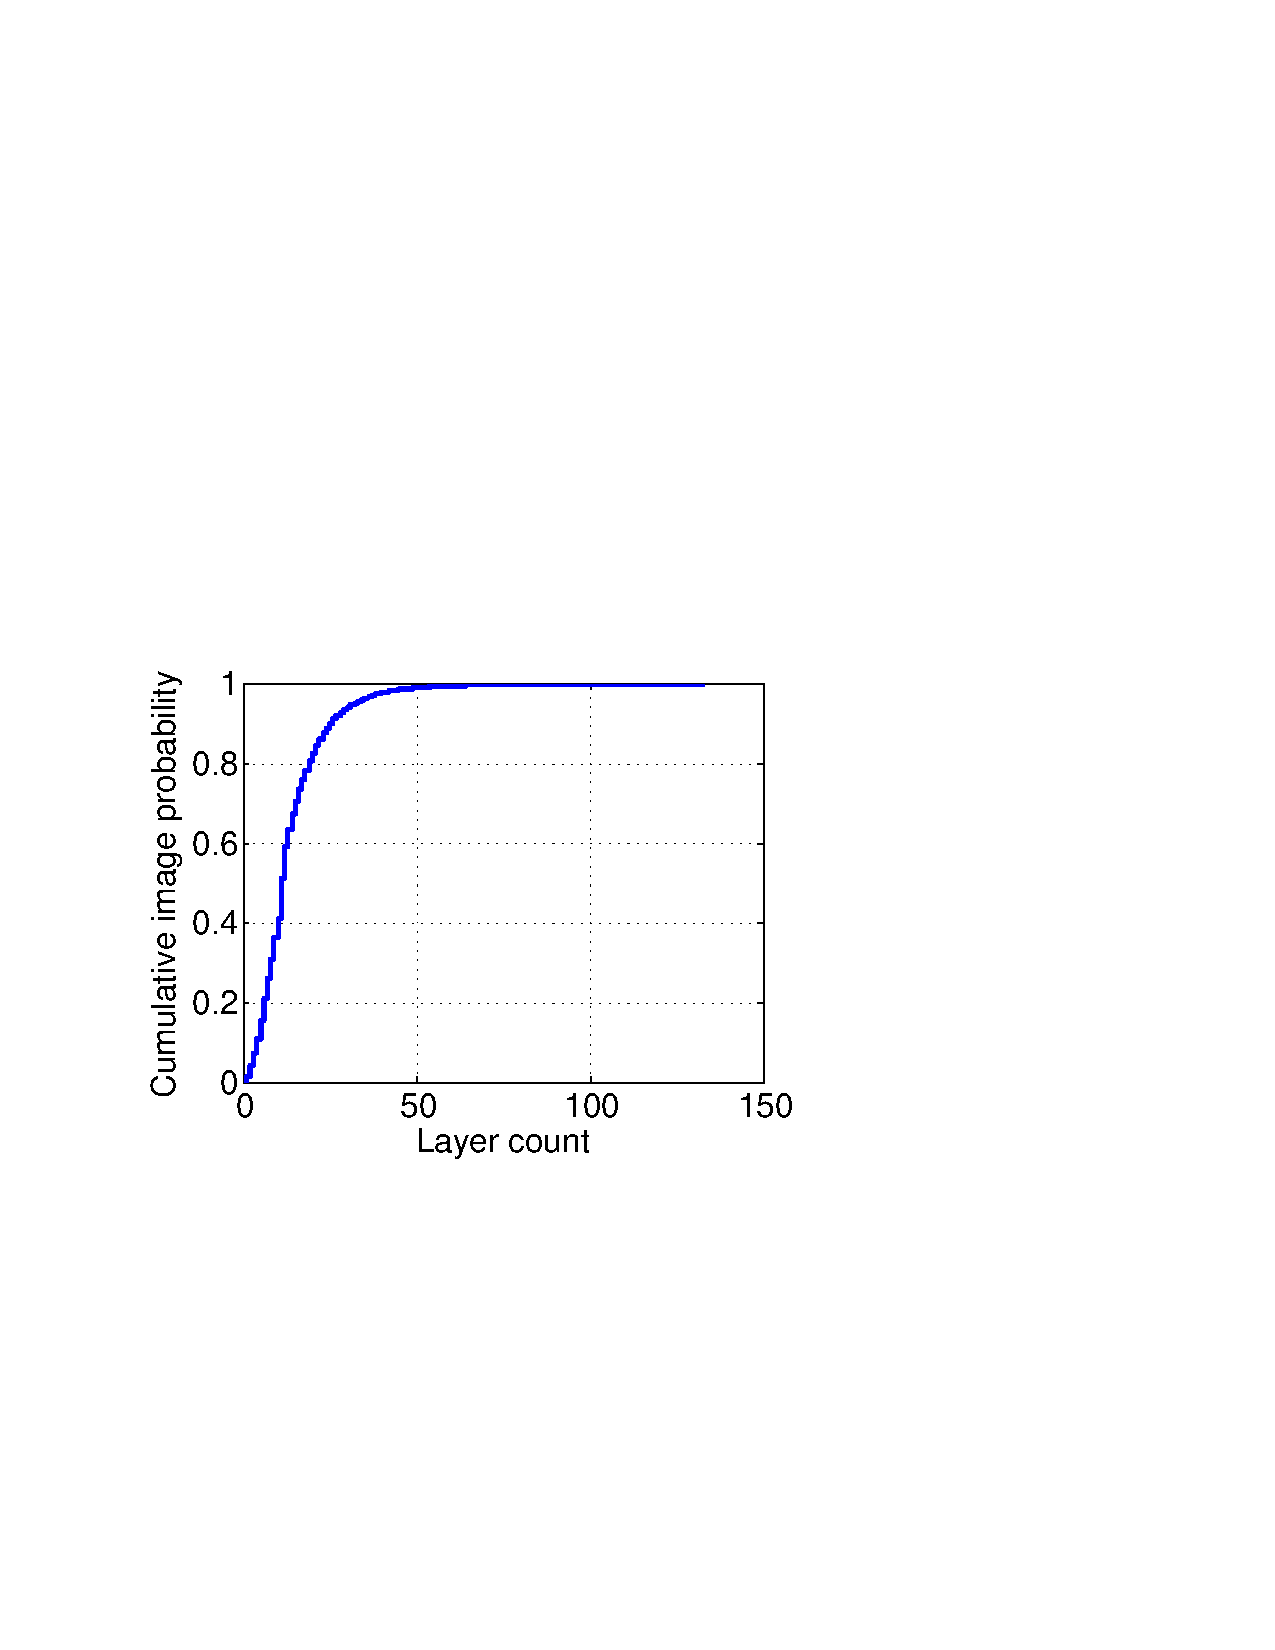
\includegraphics[width=0.215\textwidth]{graphs/image-layer-cnt}%
	}
	\subfigure[Histogram of layer count]{\label{fig:hist_layer_count}
		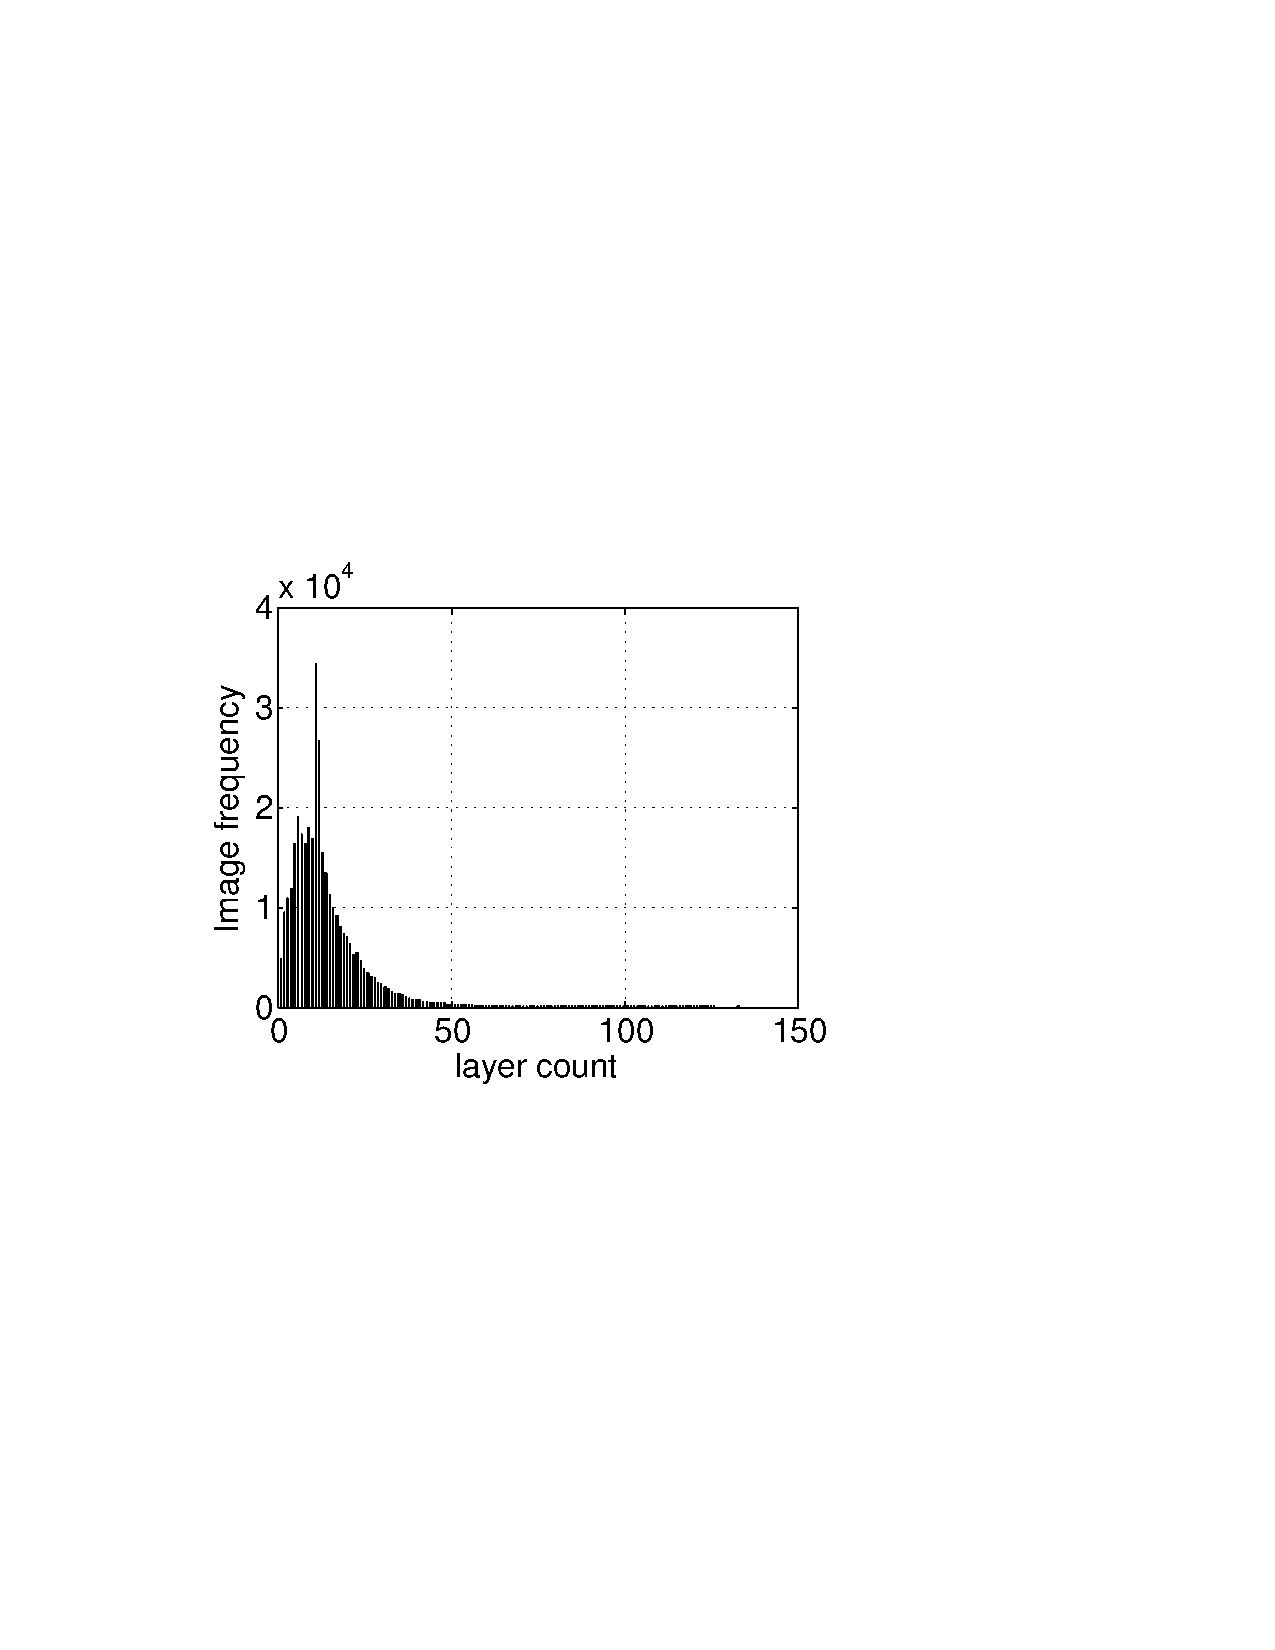
\includegraphics[width=0.21\textwidth]{graphs/image-layer-cnt-pdf.pdf}
	}
	\caption{CDF and histogram of Layer count per image.}
	\label{fig:image-size}
\end{figure}


As discussed in~\ref{sec:layers}, images consist of a set of layers.
%
It is important to understand the layer count of the images as previous work
found that the number of layers can impact the performance of I/O
operations~\cite{slacker}.
%
Therefore, we count the number of layers per image and plot the CDF (see
Figure~\ref{fig:layer_count}) and layer count frequencies (see
Figure~\ref{fig:hist_layer_count})for all Docker Hub images.

The results show that 90\% of the images have less than 26 layers while half of
the images have less than 10 layers.
%
11 layers is also the most frequent layer value with 34,420 images consisting
of exactly 11 layers.
%
The maximum layer count is 120 in the \textit{cfgarden/120-layer-image}.
%
We also find that there are 4,792 images which only consist of a single layer.

\emph{As a rule of thumb, less number of layers is better for the union file
system as it then needs to handle less metadata. However, as a tradeoff,
reducing the number of layers significantly effects the data sharing among
images.
%As a result, we see less number of layers shared among different
images.
%
For an example, if a image consists of only single layer its data can not be
shared with other images.}

%\begin{figure}[!t]
	\centering
	\subfigure[CDF of layer reference count]{\label{fig_repeate_layer}
		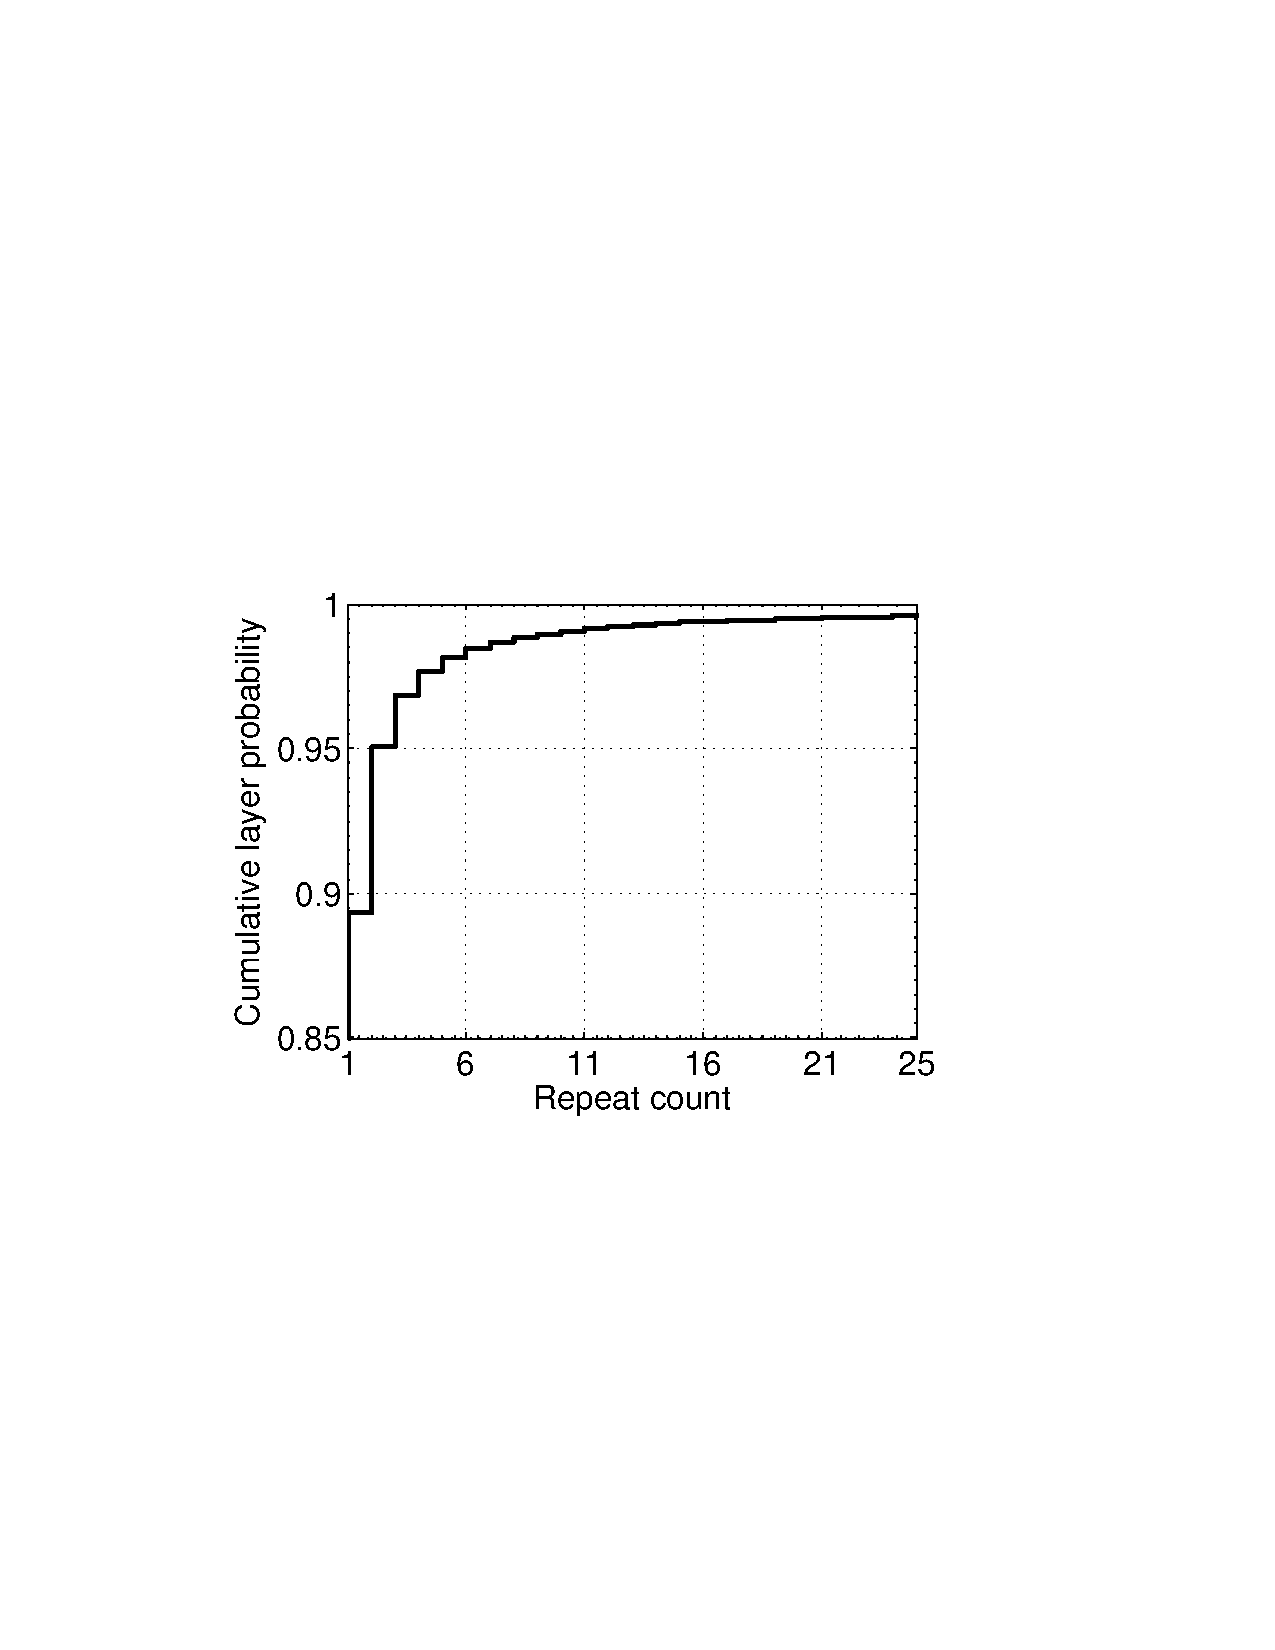
\includegraphics[width=0.23\textwidth]{graphs/repeate_layer.pdf}
	}
	\subfigure[Histogram of layer reference count]{\label{fig_hist_repeate_layer}
		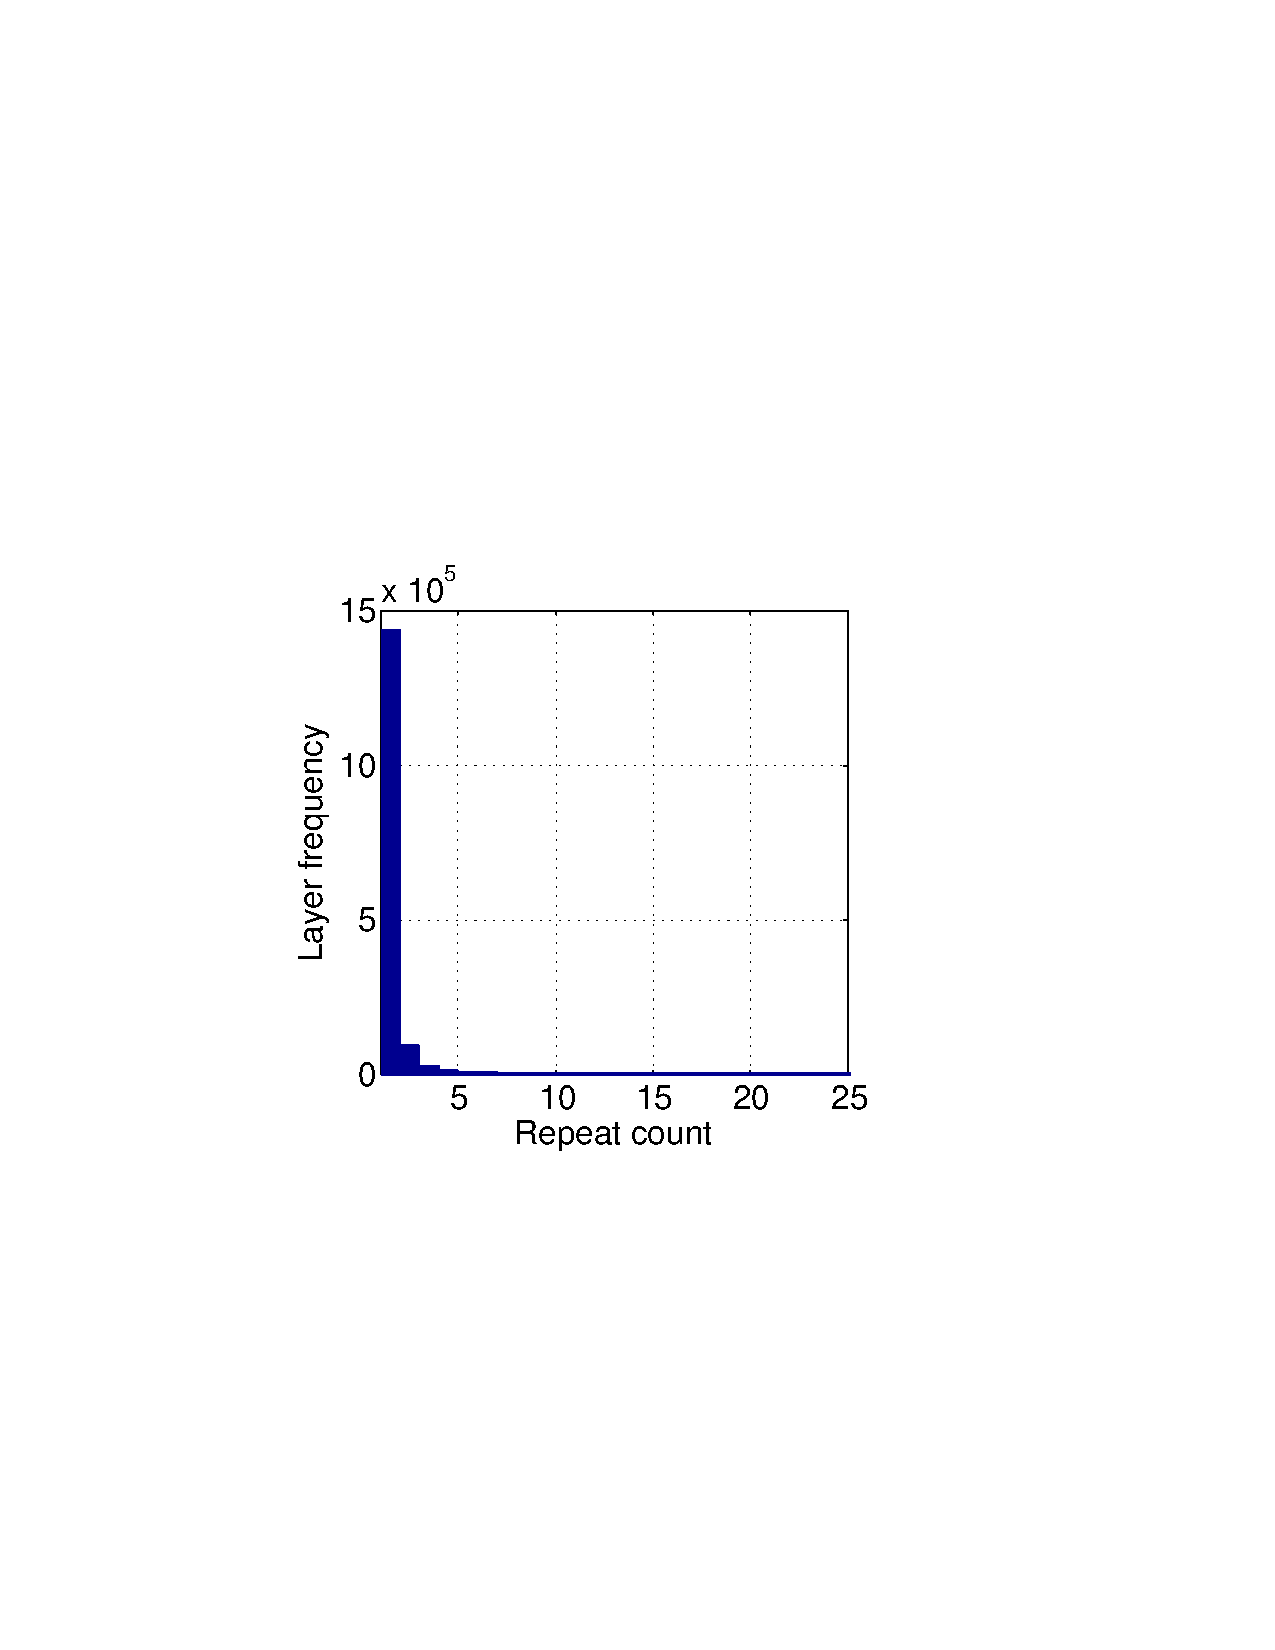
\includegraphics[width=0.223\textwidth]{graphs/hist_repeate_layer.pdf}
	}
	\caption{Layer reference counts across all images}
	\label{fig-repeat-layer-cnt}
\end{figure}

\paragraph{Layer reference count}

\begin{figure}
	\centering
	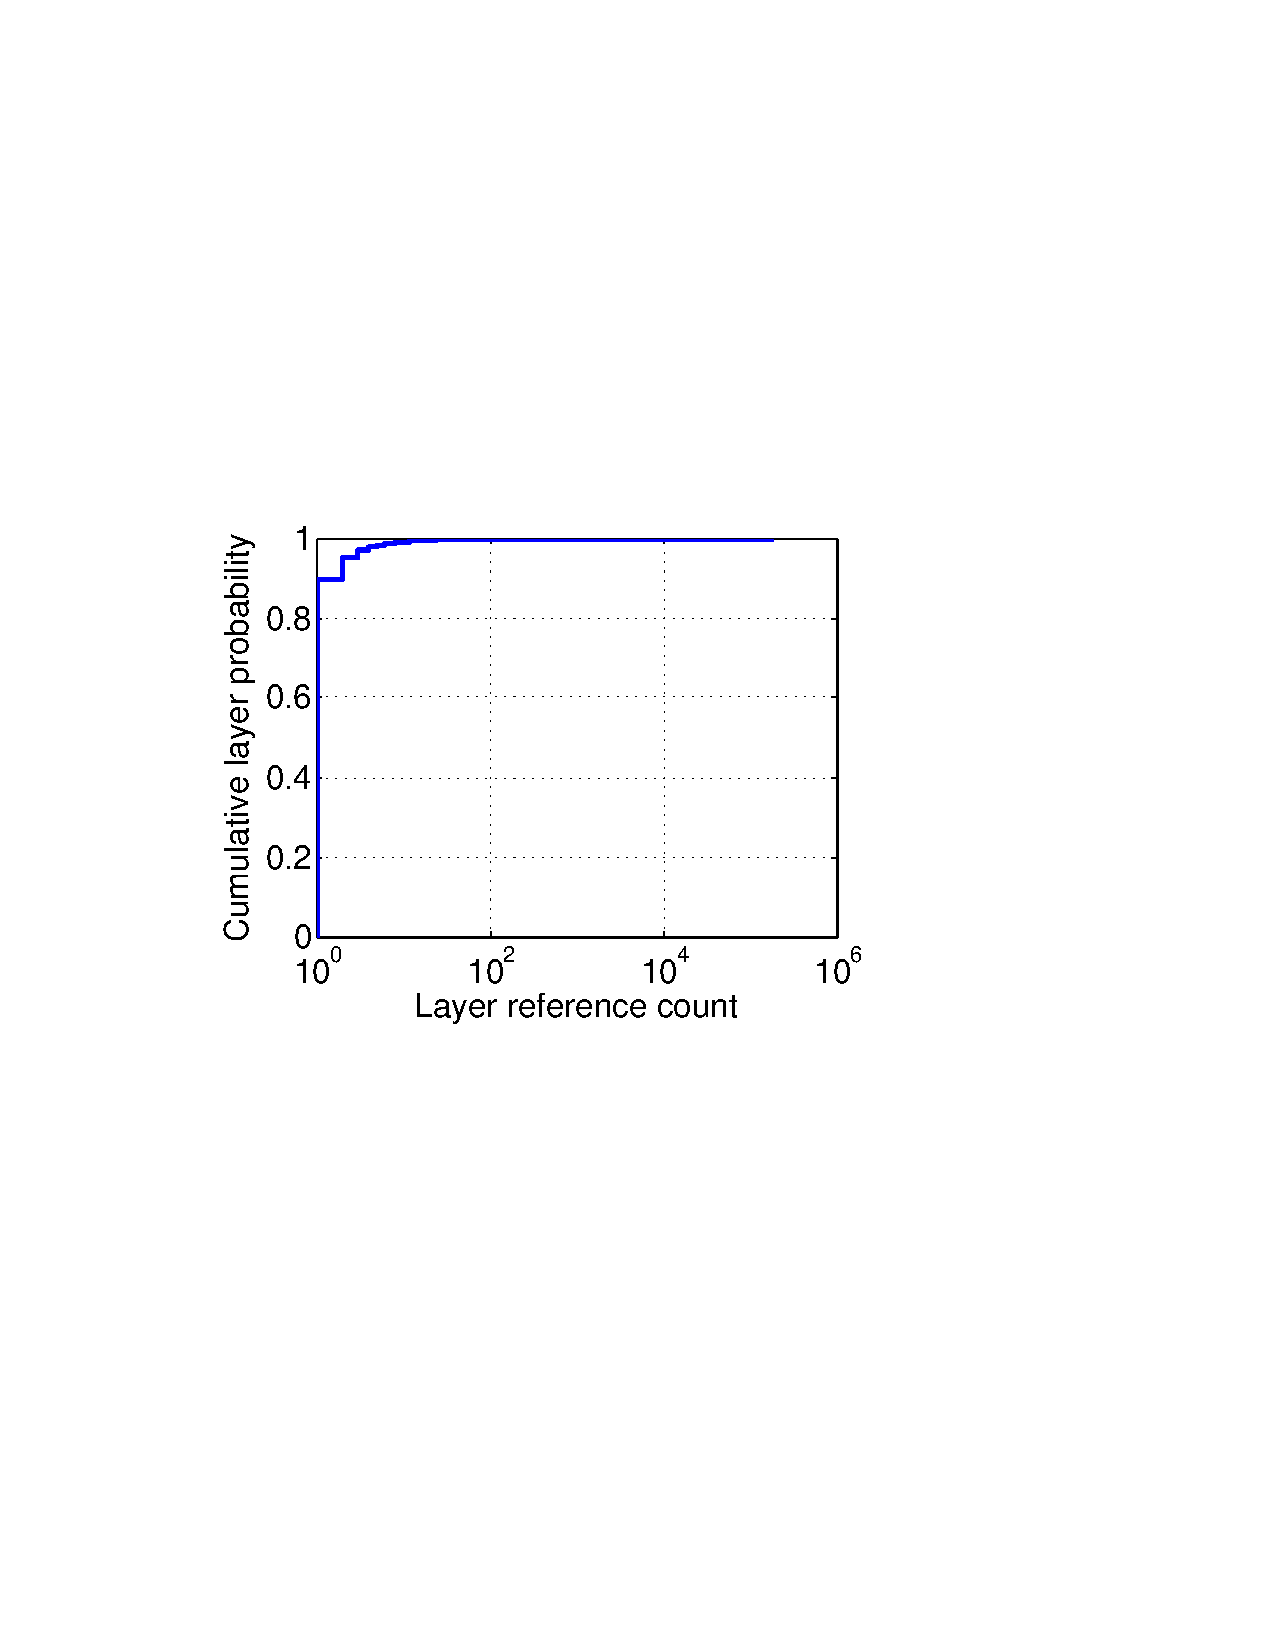
\includegraphics[width=0.21\textwidth]{graphs/shared-cnt-cdf.pdf}
	\caption{CDF of layer reference count.
	}
	\label{fig:ref_count}
\end{figure}


An interesting question is what is the sharing rate of layers across images.
%
We analyze all image manifests and count for each layer, how many times it is
referenced by an image.
%
Figure~\ref{fig:ref_count} shows that around 90\% of layers are only reference
by a single image while 95\% are reference by not more than 2 images.
%
Similarly, 99\% of layers are shared among less than 25 images. 
%
%Figure~\ref{} shows the absolute values, revealing that almost 1.5 million
%images are only referenced once.  \acomment{Figure is missing} While there is
%again a large spectrum of reference counts, the maximum is 33,428, the vast
%majority of layers is not shared. 
%
This hints that the layer-based approach to improve storage efficiency is
barely utilized and there is room for improvement in how to construct more
sharable layers.
%
\emph{These findings reveal that layer level CAS has not been very successful
and most of the layers that exists in Docker Hub are not shared among images.
%
Hence, there is a dire need of a better redundancy management.}

%89\% of 1
%95.1\% 2

\paragraph{Directory count and File count}

Next, we look at the directory (Figure~\ref{fig:dir-cnt-cdf}) and file count
(Figure~\ref{fig:file-cnt-cdf}) in images to determine if deploying images
requires handling of large amounts of metadata.
%
Looking at directories, we see that 50\% of images have less than 3,326
directories and 90\% of images have less than 9,692 directories.
%
%70\% of images have more than 2,500 directories. 
For files, 50\% of images have less than 27,194 files and 90\% of images have
less than 74,266 files.

This is consistent with our analysis of layer-based file and directory counts
and the number of layers per image.
%
Again, \textit{we conclude that most images do not require an extensive amount
of metadata when being deployed as file and directory counts are low except for
few outliers.}

%This is consistent with our analysis of layer-based file and directory counts
%and the number of layers per image. Again, we conclude that most images do not
%require an extensive amount of metadata when being deployed as file and
%directory counts are low except for few outliers.

%\begin{figure}[!t]
	\centering
	\subfigure[CDF of compression ratio]{\label{fig_cdf_compression_ratio}
		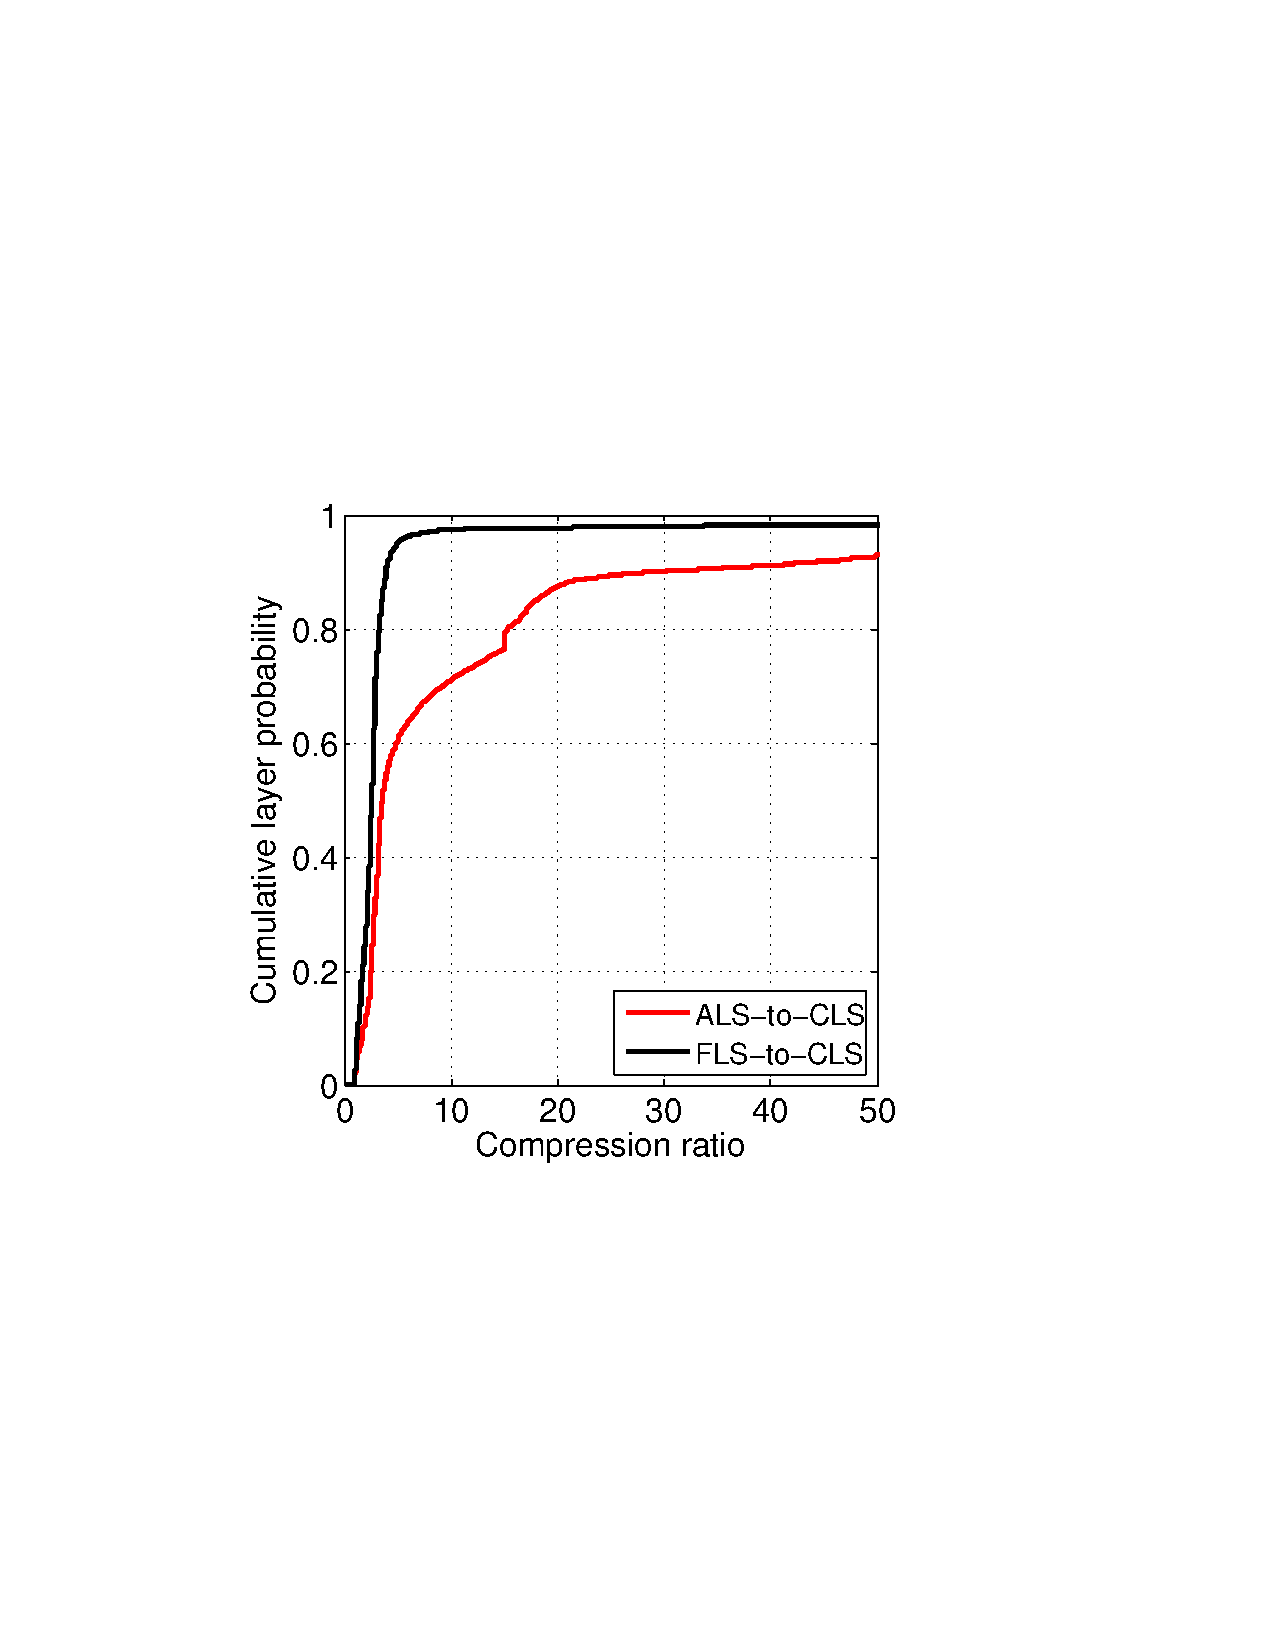
\includegraphics[width=0.23\textwidth]{graphs/cdf_compression_ratio.pdf}
	}
	\subfigure[Histogram of comp. ratios]{\label{fig_his_compression_ratio}
		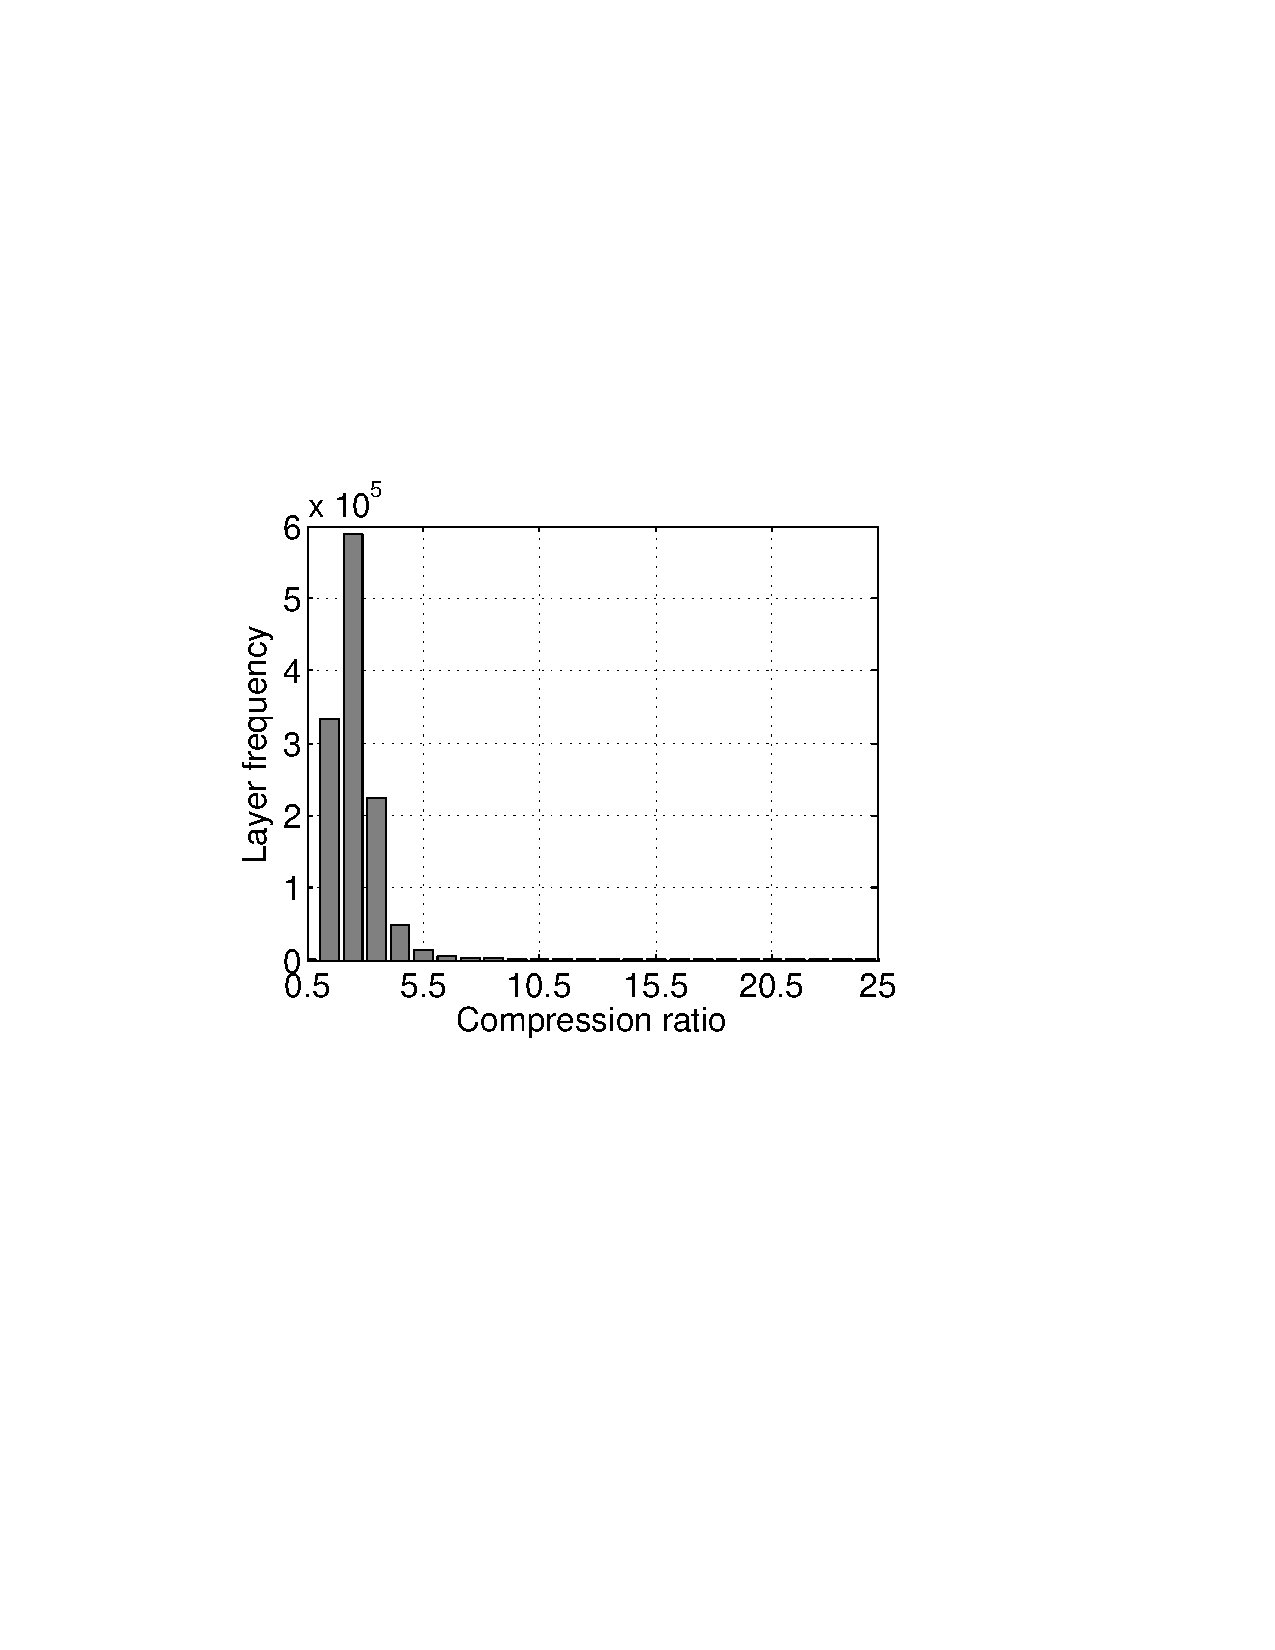
\includegraphics[width=0.223\textwidth]{graphs/his_compression_ratio.pdf}
	}
	\caption{Layer compression ratio distribution
	%\vcomment{Different colors are used in figure (a) and (b) FLS/CLS\nancomment{will address later}}
	}
	\label{fig-compression-ratio}
\end{figure}


%\paragraph{Layer compression ratios}
